\documentclass[a4paper,11pt]{article}
\usepackage{exptech}
\usepackage{textcomp}
\usepackage{graphicx}
\usepackage{array}
\usepackage[babel=true]{csquotes}
\usepackage{url}
\usepackage{hyperref}
\usepackage{wrapfig}
\usepackage[export]{adjustbox}
\usepackage{titletoc}

\hypersetup{
  bookmarks=true, % show bookmarks bar?
  pdftitle={Avalon - Documentation utilisateur}, % title
  pdfnewwindow=true, % links in new window
  colorlinks=true, % false: boxed links; true: colored links
  linkcolor=black, % color of internal links (change box color with linkbordercolor)
  citecolor=cyan, % color of links to bibliography
  filecolor=cyan, % color of file links
  urlcolor=cyan % color of external links
}

\title{
  \textbf{Avalon}\\
  Rapport de pré-étude
}
\markright{Avalon - Documentation utilisateur}
\author{
\begin{minipage}{0.4\textwidth}
	\begin{flushleft} \large
		\emph{Auteurs :}\\
		Alexandre \textsc{Audinot}\\
		Julien \textsc{Bouvet}\\
		Cyrille \textsc{Delabre}\\
		Thierry \textsc{Gaugry}\\
		Nicolas \textsc{Hurman}\\
		Léo \textsc{Jacoboni}\\
		Alexandre \textsc{Leonardi}\\
	\end{flushleft}
\end{minipage}
\begin{minipage}{0.4\textwidth}
	\begin{flushright} \large
		\emph{Encadrants :} \\
		Valérie \textsc{Gouranton}\\
		Ronan \textsc{Gaugne}\\
		Bruno \textsc{Arnaldi}\\
		Willy \textsc{Allègre}\\
		Jean-Paul  \textsc{Departe}\\
	\end{flushright}
\end{minipage}
}

\date{29 mai 2015}

\begin{document}
\maketitle
\thispagestyle{empty}
\begin{abstract}
Documentation technique à l'attention du centre de Kerpape : comment modifier le projet, détails d'implémentation, création d'une configuration MiddleVR. 
\end{abstract}

%\vfill
%[width=\textwidth]
\begin{figure}[h!]
   \begin{minipage}{0.3\linewidth}
      
\includegraphics[scale=0.9]{1-PreEtude/img/logo_insa.jpeg}
   \end{minipage} 
   \begin{minipage}{0.2\linewidth}
      \centering
      
\includegraphics[scale=0.5,left]{1-PreEtude/img/logo_irisa.jpg}
   \end{minipage}\hfill
   \begin{minipage}{0.2\linewidth}
      
\includegraphics[scale=0.9]{1-PreEtude/img/logo_kerpape.png}
   \end{minipage}
\end{figure}

\pagebreak

\tableofcontents
\pagebreak


\section{Introduction}

% Annonce plan
% Visite kerpape
% Rencontre clients
\begin{wrapfigure}{r}{0mm}
	\centering
	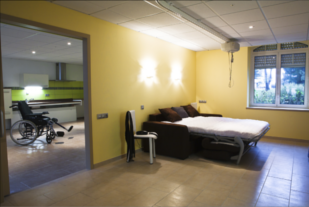
\includegraphics[scale=1]{1-PreEtude/img/appt_tremplin_intro.png}
\end{wrapfigure}
Notre projet consiste en la modélisation d'appartements tremplins en 3D pleinement interactifs, dans lesquels des personnes handicapées pourront évoluer et apprendre à se servir des différents équipements de domotique présents. 
Le projet est proposé par le centre de rééducation de Kerpape et par l'IRISA, ce qui lui confère un intérêt particulier à nos yeux car le commanditaire est extérieur à l'école, et le projet répond donc au besoin d'un véritable client de la même manière que le ferait un projet rencontré dans notre vie professionnelle. 
Ainsi, nous avons eu l'occasion de nous entretenir avec Willy Allègre et Jean-Paul Departe, ingénieurs de Kerpape à l'origine du projet, tout d'abord lors d'une conférence téléphonique pendant laquelle ils nous ont décrit ce qu'ils attendaient de l'application. Par la suite, un déplacement au centre de Kerpape nous a permis de parfaire l'image que nous nous faisons du résultat attendu et de compléter le cahier des charges de la future application. \newline

\begin{wrapfigure}{l}{0mm}
	%\cite{archeologie}
	\centering
	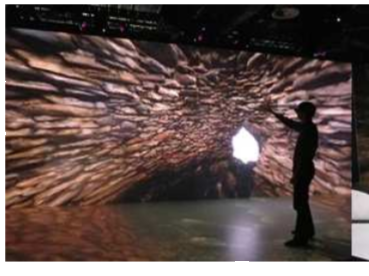
\includegraphics[scale=0.5]{1-PreEtude/img/rv_2.png}
\end{wrapfigure}
Au cours de cette étude de pré-spécifications, nous commencerons par définir plus précisément le contexte de notre projet, en tentant de cerner ce qu'est la réalité virtuelle et son importance dans le domaine de la santé. 
Nous présenterons ensuite le cahier des charges en deux parties, d'abord d'un point de vue fonctionnel, les différentes fonctions qui sont attendues de notre applications, et ensuite d'un point de vue technique, les différentes contraintes que nous aurons à respecter. 
Après cela nous décrirons, dans l'étude fonctionnelle, les différents scénarios types qui nous ont été proposés par Kerpape et auxquels les patients devront pouvoir être confrontés. 
Puis nous spécifierons les différents logiciels à notre disposition ainsi que les différents matériels, et les périphériques que nous prévoyons de rendre utilisables. 
Enfin, nous ébaucherons une planification prévisionnelle du travail à fournir tout au long de l'année. 
\pagebreak
\input{doc_technique/modifier.tex}
\pagebreak
\input{doc_technique/implementation.tex}
\pagebreak
\input{doc_technique/middlevr.tex}
\pagebreak
\section{Conclusion}

Nous avons donc choisi une méthode fortement inspirée du cycle de production en V mais en la mêlant à des méthodes agiles pour pouvoir présenter le projet à nos clients régulièrement. Ainsi si chaque jalon du projet, représenté par un livrable à rendre, correspond à une étape de notre cycle en V, nous prévoyons en parallèle d'avancer le développement de l'application, en en présentant les itérations successives à Jean-Paul Departe et Willy Allègre. \newline

Ainsi, nos commanditaires peuvent valider notre avancée en quasi-temps réel. De plus, d'après l'audit réalisé sur Microsoft Project, nous disposons d'une planification correcte. Les différents livrables seront réalisés dans les temps et les estimations que nous avons faites tiennent compte des contre-temps que nous sommes susceptibles de rencontrer et devraient suffire à absorber les retards.
\pagebreak
\bibliography{1-PreEtude/biblio}

\end{document}
